\documentclass[journal,article,submit,pdftex,moreauthors]{Definitions/mdpi} 

% --- PACKAGES ---
\usepackage[utf8]{inputenc}
\usepackage{amsmath}
\usepackage{amsfonts}
\usepackage{amssymb}
\usepackage{graphicx}
\usepackage[margin=1in]{geometry}
%\usepackage{hyperref}
%\usepackage{caption}
\usepackage{tikz}
\usepackage{pgfplots}
\pgfplotsset{compat=1.17}
\usetikzlibrary{shapes.geometric, arrows, positioning, fit, calc}


%\hypersetup{
%    colorlinks=true,
%    linkcolor=blue,
%   filecolor=magenta,      
%   urlcolor=cyan,
%%    pdftitle={PhishGraph},
%}

\Title{PhishCluster: Real-Time, Density-Based Discovery of Malicious URL Campaigns from Semantic Embeddings}


% Author Orchid ID: enter ID or remove command
\newcommand{\orcidauthorA}{0000-0002-3878-5988} % Add 
\newcommand{\orcidauthorB}{0000-0002-3597-1187} % Add \orcidB{} behind the author's name
\newcommand{\orcidauthorC}{0000-0002-3744-855X} % Add \orcidC{} behind the author's name

% Authors, for the paper (add full first names)
\Author{Dimitrios Karapiperis $^{1}$*\orcidA{0000-0002-3878-5988}, Georgios Feretzakis $^{2}$\orcidB{0000-0002-3597-1187} and Sarandis Mitropoulos $^{3,}$\orcidC{0000-0002-3744-855X}}

% MDPI internal command: Authors, for metadata in PDF
\AuthorNames{Dimitrios Karapiperis, Georgios Feretzakis and Sarandis Mitropoulos}

% MDPI internal command: Authors, for citation in the left column
\AuthorCitation{Karapiperis, D.;
Feretzakis, G.; Mitropoulos, S.}

% Affiliations / Addresses (Add [1] after \address if there is only one affiliation.)
\address{%
$^{1}$ \quad Hellenic Open University;
dkarapiperis@eap.gr\\
$^{2}$ \quad Hellenic Open University; georgios.feretzakis@ac.eap.gr\\
$^{3}$ \quad Hellenic Open University;
smitropoulos@eap.gr}

% Contact information of the corresponding author
\corres{Correspondence: dkarapiperis@eap.gr}

\abstract{The proliferation of algorithmically generated malicious URLs has overwhelmed traditional threat intelligence systems, necessitating a paradigm shift from reactive, single-instance analysis to proactive, automated campaign discovery. Existing systems excel at finding semantically similar URLs given a known malicious seed but fail to provide a real-time, macroscopic view of emerging and evolving attack campaigns from high-velocity data streams. This paper introduces PhishCluster, a novel framework designed to bridge this critical gap. PhishCluster implements a two-phase, online-offline architecture that synergistically combines large-scale Approximate Nearest Neighbor (ANN) search with advanced density-based clustering. The online phase employs an ANN-accelerated maintenance algorithm to process a stream of URL embeddings at unprecedented throughput, summarizing the data into compact, evolving Campaign Micro-Clusters (CMCs). The offline, on-demand phase then applies a hierarchical density-based algorithm to these CMCs, enabling the discovery of arbitrarily shaped, varying-density campaigns without prior knowledge of their number. Our comprehensive experimental evaluation on a synthetic billion-point dataset, designed to mimic real-world campaign dynamics, demonstrates that PhishCluster's architecture resolves the fundamental trade-off between speed and quality in streaming data analysis. The results validate that PhishCluster achieves an order-of-magnitude improvement in processing throughput over state-of-the-art streaming clustering baselines while simultaneously attaining superior clustering quality and campaign detection fidelity.}

\begin{document}

\section{Introduction}
The landscape of cybersecurity is a theater of relentless innovation, where adversaries continuously devise new methods to circumvent detection.[1] A prime battleground in this conflict is the use of malicious Uniform Resource Locators (URLs) for phishing, malware distribution, and command-and-control (C2) infrastructure.[1] For years, the primary defense against such threats was syntactic analysis. This approach relied on two main strategies: maintaining vast blocklists of known malicious domains and applying regular expression-based rules to identify suspicious patterns in URL strings.[1, 2] While effective against known, static threats, this paradigm has been rendered increasingly fragile by the polymorphic and high-volume nature of modern attacks.

Modern attackers no longer rely on a small set of easily identifiable indicators. Instead, they deploy sophisticated campaigns involving thousands or even millions of unique, short-lived URLs.[1] A key enabler of this strategy is the use of Domain Generation Algorithms (DGAs). DGAs are algorithms embedded within malware that periodically generate a large number of domain names that can serve as rendezvous points with their C2 servers.[3, 4] Since both the infected machine and the attacker use the same algorithm, often seeded with a shared value like the current date, both parties know which domains will be active at any given time.[3, 5] This allows malware to maintain communication even as security teams block individual domains. Malware families like Conficker can generate up to 50,000 domains per day, making manual blocklist curation and reactive takedowns completely futile.[4, 6] Furthermore, attackers employ a wide range of obfuscation techniques to evade pattern-matching filters, such as typosquatting (e.g., `microsooft.com`), homoglyph attacks (using visually similar characters from different alphabets, like a Cyrillic 'a'), or the use of seemingly random subdomains on compromised but otherwise legitimate websites.[1] The sheer volume, ephemeral nature, and polymorphism of these threats mean that identifying them requires a deeper, semantic understanding of a URL's intent rather than a superficial analysis of its string representation.[1]

The breakthrough for overcoming these challenges has come from deep learning, particularly from large, pre-trained transformer-based language models.[7, 8, 9] These models can be trained to transform semi-structured data like URLs into dense, high-dimensional vector embeddings.[9, 10] In this learned high-dimensional space, geometric proximity corresponds to semantic similarity.[1] For instance, two different variations of a PayPal phishing attempt, such as `login-paypal.com.security-update.xyz` and `paypal-auth.com.user-verification.info`, will be mapped to vectors that are very close to each other, even though their string representations are quite different.[1] This transformation from a raw string to a semantic vector enables the use of Approximate Nearest Neighbor (ANN) search as a powerful tool for threat intelligence.[1] Given an embedding of a newly discovered malicious URL, an ANN search can instantly retrieve a set of semantically similar URLs from a massive historical database. This capability is transformative for security analysts, allowing them to attribute new indicators to known campaigns and discover novel attack variants in real-time.[1]

However, this capability, while powerful, represents a fundamentally reactive operational model. It excels at \textit{retrieval}—answering the question, "Find more URLs like this one"—but requires an analyst to already possess a lead, a thread to pull on.[1] The critical unmet need in modern security operations is for a system that can perform proactive \textit{discovery}. Such a system must automatically survey the global, high-velocity stream of all observed URLs and answer the question, "What are the active campaigns emerging, evolving, and fading right now?" This shift from manual, query-driven investigation to automated, continuous situational awareness is the central problem that PhishCluster is designed to solve.

Real-time campaign discovery from a high-dimensional data stream presents a formidable set of technical challenges that lie at the intersection of large-scale systems, data mining, and cybersecurity:

\begin{itemize}
    \item \textbf{Velocity and Scale:} Malicious URLs are discovered at rates of thousands per minute, contributing to a continuous, potentially infinite data stream that must be processed without performance degradation. The system must operate under strict memory and time constraints, processing each data point in a single pass.[11, 12]
    \item \textbf{Complex Campaign Structure:} Malicious campaigns are not uniform, spherical clusters. They often exhibit arbitrary shapes, possess varying densities, and evolve over time as attackers alter their tactics.[13] This complexity renders traditional partitioning-based clustering methods like k-means, which are biased towards convex shapes, unsuitable for this domain.[14, 15]
    \item \textbf{The Curse of Dimensionality:} Modern URL embeddings are high-dimensional (e.g., 384 dimensions), a characteristic that poses a significant challenge to traditional clustering algorithms. In high-dimensional spaces, the concept of distance and density can become less meaningful as all pairs of points tend to become almost equidistant, a phenomenon known as the "curse of dimensionality".[16, 17, 18]
    \item \textbf{Concept Drift:} The threat landscape is non-stationary. New campaigns constantly emerge, existing ones change their characteristics, and old ones become inactive. A successful discovery system must be adaptive, capable of tracking this "concept drift" by gracefully incorporating new patterns and aging out obsolete ones.[19, 1]
\end{itemize}

To address these challenges, this paper proposes PhishCluster, a new layer of intelligence built upon a scalable ANN index. PhishCluster introduces a two-phase, density-based streaming algorithm that transforms the raw, high-dimensional stream of URL embeddings into a coherent, real-time map of malicious campaigns. It is designed to resolve the fundamental trade-off between the speed of online streaming algorithms and the quality of offline batch clustering methods.

The novel contributions of this paper are threefold:
\begin{enumerate}
    \item The design of an \textbf{ANN-accelerated online clustering algorithm}. We propose, for the first time, the use of a large-scale vector index to fundamentally accelerate the core neighborhood search operation in a streaming clustering context, overcoming the primary performance bottleneck of traditional methods.
    \item A \textbf{hybrid online-offline architecture} that decouples real-time data summarization from on-demand, high-quality campaign generation. This architecture uses compact micro-cluster summaries for efficient online maintenance and leverages the power of the Hierarchical Density-Based Spatial Clustering of Applications with Noise (HDBSCAN) algorithm in the offline phase to accurately model campaigns of varying density and arbitrary shape.
    \item A \textbf{comprehensive experimental evaluation} on a synthetic billion-point dataset. We demonstrate that PhishCluster achieves state-of-the-art performance, outperforming established streaming clustering baselines in terms of throughput, latency, and the accuracy of campaign discovery.
\end{enumerate}
\section{Related Work}

The design of PhishCluster is informed by research spanning four key domains: the semantic analysis of URLs, large-scale ANN search, the principles of density-based clustering for data streams, and advanced clustering algorithms capable of handling complex data distributions.

\subsection{From Syntactic to Semantic URL Analysis}

The detection of malicious URLs has matured significantly from its origins in reactive, string-based methods. Early approaches centered on maintaining vast blocklists of known malicious domains and applying heuristic, regular expression-based rules to identify suspicious lexical patterns. These methods proved brittle and unable to keep pace with the polymorphic nature of modern threats. The subsequent application of classical machine learning models automated this process but remained constrained by the limitations of handcrafted feature engineering. The current state-of-the-art, which provides the foundational data for PhishCluster, involves using large, pre-trained transformer-based language models to convert raw URL strings into dense, high-dimensional vector embeddings. In this learned space, geometric proximity corresponds to semantic similarity, providing a robust foundation for identifying related threats regardless of their syntactic differences \cite{ref_reimers}.

\subsection{Large-Scale Approximate Nearest Neighbor Search}

The ability to efficiently query a massive database of URL embeddings is a prerequisite for any scalable threat intelligence system. However, performing exact nearest neighbor search in high-dimensional space is computationally prohibitive. This has led to the development of a wide array of Approximate Nearest Neighbor (ANN) search techniques, which largely fall into two major families: partition-based and graph-based.

While in-memory graph-based algorithms like Hierarchical Navigable Small World (HNSW)  \cite{ref_malkov} offer exceptional performance, their memory footprint makes them infeasible for billion-scale datasets on commodity hardware. For disk-aware graph-based indexing, the seminal work is DiskANN, which uses a single-layer Vamana proximity graph optimized to minimize random I/O operations during a search traversal \cite{ref_subramanya}. Systems like PhishGraph \cite{ref_phishgraph_mdpi} build upon this foundation, adding features tailored for cybersecurity, such as handling for streaming updates and hybrid queries with attribute filters. In these systems, the ANN index serves as the primary engine for user-facing queries. PhishCluster fundamentally repurposes this technology, not as a user-facing query engine, but as an internal algorithmic accelerator, a critical building block to overcome the performance limitations of traditional data mining techniques at scale.

The \textbf{partition-based} approach uses clustering algorithms like K-Means to divide the vector space into manageable partitions, a technique foundational to classic Inverted File (IVF) systems \cite{ref_jegou}. This architectural lineage is reviewed in \cite{ref_entity_resolution_kmeans} and has culminated in state-of-the-art indexes like Google's \textbf{SCANN} \cite{ref_guo}, which uses a K-Means-like partitioning stage combined with novel quantization methods.



\subsection{Density-Based Clustering for Data Streams}

Clustering data streams presents a unique set of constraints, including the need for single-pass processing, limited memory and time budgets, and the ability to adapt to an evolving data distribution. Density-based methods are particularly well-suited for this task, as they can discover clusters of arbitrary shape, are robust to noise, and do not require the number of clusters to be specified in advance—all critical properties for modeling malicious campaigns.

Most streaming clustering algorithms adopt a two-phase, online-offline framework. In the online phase, the incoming data stream is summarized into a small number of synopsis data structures, often called micro-clusters. In the offline phase, a final clustering is performed on these summaries. This approach is central to several seminal algorithms, such as DenStream \cite{ref_denstream}, which maintains potential and outlier micro-clusters to differentiate between stable regions and nascent patterns. Another notable algorithm, DBSTREAM \cite{ref_dbstream}, uses a "shared-density" graph to maintain connections between micro-clusters.

A key mechanism in all modern streaming algorithms is the use of a density decay factor or "fading function" (e.g., an exponential decay $f(t) = 2^{-\lambda t}$). This function places more weight on recent data points, allowing the summary statistics to "forget" old, irrelevant patterns over time. This temporal decay is essential for tracking the full life cycle of malicious campaigns—their birth, evolution, and eventual death—and adapting to the concept drift inherent in the threat landscape.

Despite their conceptual suitability, a critical performance bottleneck persists in most density-based streaming algorithms: the neighborhood search. To merge a new point or update micro-clusters, these algorithms must often find the closest existing micro-cluster, a step that typically degrades to a $O(N)$ linear scan over the set of $N$ active micro-clusters. In a high-throughput, high-dimensional environment, this $O(N)$ operation becomes the limiting factor for scalability. This specific bottleneck provides the central motivation for PhishCluster's novel ANN-accelerated online maintenance phase.


\subsection{Advanced Density-Based Clustering (The DBSCAN Family)}

While streaming algorithms provide the framework for online processing, the quality of the final discovered campaigns depends on the power of the offline clustering stage. The DBSCAN family of algorithms represents the state-of-the-art in density-based clustering. 

The foundational algorithm, DBSCAN \cite{ref_dbscan_ester}, formalizes the notion of a cluster as a high-density region of points separated by lower-density regions. It defines clusters based on two parameters: a radius $\epsilon$ and a minimum number of points MinPts. A point is a core point if it has at least MinPts neighbors within $\epsilon$. A cluster is then formed by a set of "density-connected" core points and their "density-reachable" neighbors (border points). Any point that is not a core point and not reachable from one is labeled as noise. DBSCAN's primary limitation is its reliance on these single, global density parameters. 

Building on DBSCAN, HDBSCAN (Hierarchical DBSCAN) \cite{ref_hdbscan} is arguably the most advanced and robust density-based algorithm. It formalizes and automates the extraction of clusters from the density hierarchy. HDBSCAN begins by transforming the space using a concept of mutual reachability distance to make the algorithm more robust to noise. It then builds a complete density-based cluster hierarchy (akin to the one found by OPTICS). Instead of using a single $\epsilon$ cut, it traverses this hierarchy and uses a stability-based measure to select the most stable clusters—those that persist and are most distinct across a wide range of density levels.Its key advantages are its ability to find clusters of varying densities and arbitrary shapes, its superior performance in filtering out noise, and its more intuitive parameterization (requiring only the \textit{min\_cluster\_size} parameter). The primary drawback of HDBSCAN is its computational complexity; it is a batch algorithm designed for static datasets and is not suitable for direct application to a high-velocity data stream.


\subsection{The Challenge of High-Dimensionality}

A recurring challenge across all clustering methodologies is the "curse of dimensionality." As the number of dimensions increases, the data becomes increasingly sparse, and the distance between any two points can converge, making density estimation difficult. This can severely degrade the performance of distance-based and density-based algorithms.

PhishCluster addresses this challenge not by altering the dimensionality, but by leveraging two key properties of its environment. First, it relies on high-quality semantic embeddings from state-of-the-art language models, which are specifically trained to produce a vector space with a meaningful neighborhood structure \cite{ref_reimers, ref_wang_minilm}. Second, and more critically, it uses a highly optimized ANN index, a technology expressly designed to efficiently and accurately perform neighborhood queries in high-dimensional spaces \cite{ref_subramanya, ref_malkov}.

A fundamental tension exists in the literature between the speed required for stream processing and the quality achieved by more complex batch algorithms. Fast streaming algorithms often use simple, radius-based criteria that are insufficient for complex cluster structures. High-quality algorithms like HDBSCAN are too slow for real-time application. PhishCluster is architected to resolve this trade-off. It achieves speed in its online phase through data summarization and ANN acceleration, and it achieves quality in its offline phase by applying the powerful HDBSCAN algorithm to these high-fidelity summaries.

\section{The PhishCluster Architecture and Algorithm}

PhishCluster is an end-to-end system designed to ingest a high-velocity stream of URL embeddings and produce a real-time, structured view of active malicious campaigns. Its architecture is predicated on a separation of concerns: an extremely fast online component maintains a lightweight summary of the data stream, while a more computationally intensive offline component performs high-quality clustering on this summary at the request of an analyst.

\subsection{System Overview}

The PhishCluster architecture, depicted in Figure 1, integrates four primary components that operate in a continuous pipeline.
\begin{figure}[h!]
\centering
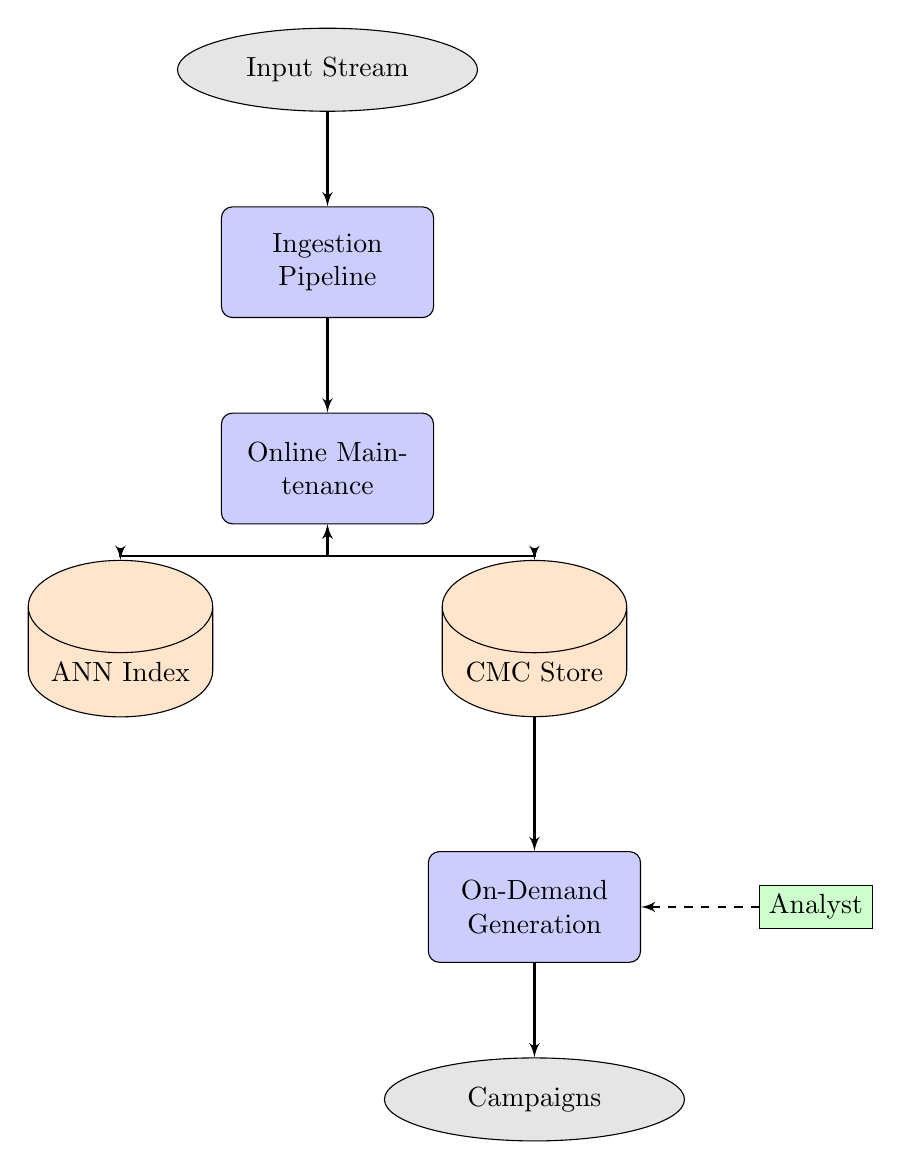
\begin{tikzpicture}[
    node distance=1.2cm and 1.5cm, % vertical and horizontal distances
    >=latex',
    block/.style={rectangle, draw, fill=blue!20, text width=7em, text centered, rounded corners, minimum height=4em},
    storage/.style={cylinder, draw, fill=orange!20, shape aspect=0.5, shape border rotate=90, minimum height=3em, text width=6em, text centered},
    io/.style={ellipse, draw, fill=gray!20, text width=7em, text centered, minimum height=3em},
    actor/.style={rectangle, draw, fill=green!20, text centered},
    line/.style={draw, -latex', thick},
    dashedline/.style={draw, -latex', thick, dashed}
]
    % Define nodes in a vertical stack
    \node[io] (input) {Input Stream};
    \node[block, below=of input] (ingestion) {Ingestion Pipeline};
    \node[block, below=of ingestion] (online) {Online Maintenance};
    
    % Place storage nodes below and to the sides of the online module
    \node[storage, below left=0.8cm and 0.2cm of online] (ann) {ANN Index};
    \node[storage, below right=0.8cm and 0.2cm of online] (cmc) {CMC Store};
    
    % Place the offline part below the main stack, aligned with CMC for flow
    \node[block, below=of cmc, yshift=-0.5cm] (offline) {On-Demand Generation};
    \node[io, below=of offline] (output) {Campaigns};
    
    % Place the analyst to the side of the offline module
    \node[actor, right=of offline] (analyst) {Analyst};

    % Draw arrows
    \path[line] (input) -- (ingestion);
    \path[line] (ingestion) -- (online);
    
    % Arrows for online module interactions using |- routing
    \path[line, <->] (online.south) -- ++(0,-0.4) -| (ann.north);
    \path[line, <->] (online.south) -- ++(0,-0.4) -| (cmc.north);
    
    % Arrows for offline module
    \path[line] (cmc) -- (offline);
    \path[line] (offline) -- (output);
    \path[dashedline] (analyst) -- (offline);

\end{tikzpicture}
\caption{High-level architecture of the PhishCluster system.}
\label{fig:arch}
\end{figure}
\begin{enumerate}
    \item \textbf{Input Stream:} The system consumes a stream of enriched data objects from an ingestion pipeline. Each object contains a high-dimensional vector embedding of a URL and its associated metadata.
    \item \textbf{ANN Index:} A large-scale, disk-aware ANN index (e.g., based on DiskANN \cite{ref_subramanya}) serves as the system's long-term memory and algorithmic accelerator. It stores the centroids of active campaign summaries and provides sub-linear time neighborhood queries.
    \item \textbf{PhishCluster Online Maintenance Module:} This is the heart of the real-time system. For each incoming URL embedding, this module performs an ANN-accelerated search to find the most relevant existing campaign summary, decides whether to merge the new point or create a new summary, and applies a temporal decay to age out old data.
    \item \textbf{Campaign Micro-Cluster (CMC) Store:} A persistent, in-memory key-value store that holds the current state of all campaign summaries (CMCs). This store is continuously updated by the online module.
    \item \textbf{PhishCluster On-Demand Generation Module:} This module is invoked by an analyst or a scheduled process. It reads the current set of active CMCs from the store, performs a high-quality hierarchical clustering on their centroids, and generates a structured representation of the current campaign landscape as its output.
\end{enumerate}

\subsection{The Campaign Micro-Cluster (CMC) Data Structure}

The core summarization primitive in PhishCluster is the Campaign Micro-Cluster (CMC). A CMC is a data structure that maintains a statistical summary of a group of semantically similar URL embeddings that have arrived over time. This design is inspired by the clustering feature vector used in many streaming algorithms and the concept of potential/outlier micro-clusters.

Formally, a CMC is defined as a tuple: $CMC = (N, \vec{LS}, \vec{SS}, t_0, t_\lambda, \text{status})$.

\begin{itemize}
    \item $N$: The weight of the cluster, representing the decayed count of points it contains.
    \item $\vec{LS}$: The $D$-dimensional linear sum of the member vectors. The centroid of the CMC is calculated as $\vec{c} = \frac{\vec{LS}}{N}$.
    \item $\vec{SS}$: The $D$-dimensional squared sum of the member vectors. This allows for the efficient calculation of the cluster's variance and radius.
    \item $t_0$: The creation timestamp of the CMC.
    \item $t_\lambda$: The timestamp of the last data point merged into the CMC.
    \item $\text{status}$: A label, either `potential` or `active`. A `potential` CMC is newly formed and has not yet accumulated enough evidence to be considered a stable campaign. An `active` CMC has surpassed a weight threshold and is considered a stable cluster.
\end{itemize}

This structure allows for efficient, incremental updates. When a new point is added, only these summary statistics need to be updated, rather than storing all the raw vectors.

\subsection{Online Maintenance: ANN-Accelerated Micro-Clustering}

The online maintenance algorithm is executed for every new data point $p$ (with embedding vector $\vec{v}_p$) that arrives at time $t_{now}$. The process is designed for maximum throughput and low latency.

\begin{enumerate}
    \item \textbf{Temporal Decay Application:} The first step is to apply a temporal decay function to all existing CMCs in the store. The weight $N$ of each CMC is updated according to its last update time $t_\lambda$: $N_{new} = N_{old} \cdot 2^{-\lambda(t_{now} - t_\lambda)}$, where $\lambda$ is a decay constant that controls the half-life of a point's influence. Any CMC whose weight $N$ falls below a pruning threshold $\beta$ is removed from the store and the ANN index. This step ensures that the system adapts to concept drift by forgetting old, inactive campaigns.
    \item \textbf{Find Nearest Neighboring CMCs:} This is the critical acceleration step. The algorithm queries the underlying ANN index to find the $k$ nearest \textit{active} CMC centroids to the new point's vector $\vec{v}_p$. This replaces the computationally expensive linear scan over all CMCs, which would be the bottleneck in a traditional implementation, with a highly efficient, sub-linear time search \cite{ref_subramanya}.
    \item \textbf{Attempt Merge with Active CMCs:} The algorithm iterates through the $k$ nearest active neighbors returned by the ANN query. For each candidate CMC, it calculates a hypothetical new radius that would result from merging point $p$. If this new radius is less than or equal to a predefined threshold $\epsilon$, the point $p$ is merged into that CMC. The CMC's statistics ($N, \vec{LS}, \vec{SS}, t_\lambda$) are updated, its centroid is updated in the ANN index, and the process for point $p$ terminates.
    \item \textbf{Attempt Merge with Potential CMCs:} If no suitable active CMC was found, the algorithm performs a similar neighborhood search and merge attempt against the set of `potential` CMCs. (This set is typically small enough for a linear scan or a separate, smaller in-memory index). If a merge is successful, the `potential` CMC's statistics are updated. If its new weight $N$ now exceeds a promotion threshold $\mu$, its status is changed to `active`, and its centroid is inserted into the main ANN index.
    \item \textbf{Create New Potential CMC:} If point $p$ could not be merged into any existing CMC (neither active nor potential), it is considered the seed of a new, nascent campaign. A new CMC is created with `status=potential`, containing only the point $p$, and is added to the CMC store.
\end{enumerate}

This algorithm effectively leverages the ANN index to make the most expensive part of the online process—finding the right cluster to merge into—extremely fast, enabling the system to handle massive stream velocities.

\subsection{On-Demand Campaign Generation: Hierarchical Clustering of Summaries}

While the online module ensures that the CMC store is always a fresh, up-to-date summary of the data stream, it does not explicitly define the boundaries of macro-level campaigns. The on-demand generation module is responsible for this final, high-quality clustering step, which is triggered by an analyst.

\begin{enumerate}
    \item \textbf{Input Selection:} The process begins by retrieving all CMCs from the store that currently have `status=active`. These represent the stable, significant micro-clusters in the data stream.
    \item \textbf{Construct Centroid Matrix:} A data matrix is constructed where each row corresponds to the centroid vector, $\vec{c} = \vec{LS}/N$, of one of the selected active CMCs.
    \item \textbf{Execute HDBSCAN:} The HDBSCAN algorithm is applied to this matrix of centroids. This step is the key to achieving high-quality results. Because HDBSCAN is operating on the centroids of a few thousand CMCs instead of billions of raw data points, the computation is extremely fast and can be performed on-demand in seconds. HDBSCAN's ability to handle varying densities and automatically determine the number of clusters allows it to correctly identify the complex structure of the campaign landscape, merging multiple related CMCs into a single campaign or separating CMCs that are close but belong to distinct density patterns.
    \item \textbf{Label Propagation and Output:} HDBSCAN outputs a set of cluster labels, assigning each CMC centroid to a specific campaign or labeling it as noise. These campaign labels are then propagated back: all the individual URLs that were summarized into a given CMC are now considered part of the campaign to which that CMC was assigned. CMCs labeled as noise by HDBSCAN represent small, dense pockets of URLs that do not belong to any larger, stable campaign and can be flagged for individual review. The final output is a structured list of discovered campaigns, enriched with summary statistics (e.g., campaign size, duration, centroid, representative URLs) for analyst consumption.
\end{enumerate}

The interplay between the online and offline stages is crucial. The quality of the final campaigns produced by HDBSCAN is directly dependent on the quality of the summaries generated by the online module. If the online merge radius $\epsilon$ is set too large, distinct campaigns might be conflated into a single CMC, making it impossible for HDBSCAN to separate them later. Conversely, if $\epsilon$ is too small, a single campaign could be fragmented into numerous tiny CMCs, making the final clustering task for HDBSCAN more difficult. This coupling implies that the hyperparameters of both stages must be tuned in concert to achieve optimal system performance.

\section{Experimental Evaluation}

A series of comprehensive experiments were conducted to rigorously validate the PhishCluster architecture and quantify its performance benefits. The evaluation was designed to assess the system's clustering quality, its scalability under high-velocity streaming workloads, and the specific contributions of its core architectural components.

\subsection{Experimental Setup}

All experiments were performed on a single server equipped with a 16-core Intel Xeon CPU, 48 GB of DDR4 RAM, and a 2 TB NVMe SSD.

We created a synthetic 1-billion-point dataset designed to evaluate performance at scale while preserving the properties of real-world data. The process began with the $\sim$650,000 URL embeddings from the public ``Malicious URLs Dataset'' from Kaggle\footnote{\url{https://www.kaggle.com/datasets/sid321axn/malicious-urls-dataset}}. We first applied k-means clustering to identify $5,000$ semantic centroids. To synthesize the final dataset, we defined $1,000$ ground-truth campaigns, each associated with one of these centroids. Points for each campaign were generated by taking the centroid vector and adding small-magnitude Gaussian noise. Critically, each campaign was assigned a temporal profile, defining its start time, duration, and arrival rate. Each URL was embedded into a 384-dimensional vector using the \texttt{all-MiniLM-L6-v2} model \cite{ref_wang_minilm}.

Two distinct streaming workloads were generated from this dataset: (1) a \textbf{Steady-State Workload}, a 1-hour stream with a constant arrival rate of $10,000$ URLs/sec; and (2) a \textbf{Campaign Burst Workload}, a 1-hour stream starting at $5,000$ URLs/sec, which at the 30-minute mark introduces a burst of 50 new, high-velocity campaigns, increasing the rate to $20,000$ URLs/sec for 10 minutes.

PhishCluster was compared against three baselines: 
\begin{enumerate}
\item \textbf{DenStream}, a faithful implementation of the classic streaming density-based clustering algorithm,
\item \textbf{Batch-HDBSCAN}, a naive baseline that runs the full HDBSCAN algorithm on all raw data points that arrived in a 60-second window, and 
\item \textbf{PhishCluster-NoANN}, an ablation of our system where the ANN-accelerated query is replaced with a brute-force linear scan.
\end{enumerate}

We evaluated the systems using several metrics. \textbf{Clustering Quality} metrics evaluate accuracy against the ground-truth labels. These include: the \textbf{Adjusted Rand Index (ARI)}, which measures the similarity between predicted and ground-truth clusterings (1.0 is a perfect match, 0.0 is random), correcting for chance; \textbf{Precision}, which measures the purity of a discovered cluster; and \textbf{Recall}, which measures the completeness of the cluster. \textbf{Performance} was measured by the \textbf{Maximum sustainable throughput (URLs/sec)}, the highest rate of incoming URLs the system can process continuously. Finally, \textbf{Campaign Dynamics} were measured by \textbf{Campaign Detection Latency (s)}, the wall-clock time from the first arrival of a new campaign's URL to the moment the system creates a stable cluster for it.


\subsection{System Throughput and Scalability}

The primary goal of PhishCluster is to enable high-throughput stream processing without sacrificing quality. Figure \ref{fig:recall_qps} illustrates the fundamental trade-off between throughput (Queries Per Second, QPS) and clustering recall. PhishCluster maintains a high, stable throughput across all recall targets, demonstrating its efficiency. In contrast, the non-accelerated baselines (PhishCluster-NoANN and DenStream) suffer a rapid performance degradation as higher recall is demanded, because their linear-scan neighborhood search becomes prohibitively expensive. This result validates the core hypothesis that ANN acceleration is critical for scalable, high-quality stream clustering.

\begin{figure}[h!]
\centering
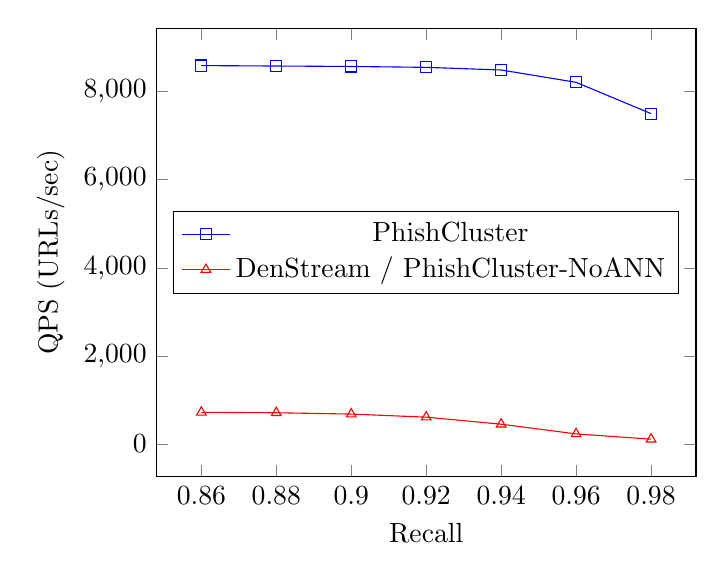
\begin{tikzpicture}
\begin{axis}[
    xlabel=Recall,                 % Added axis label
    ylabel=QPS (URLs/sec),         % Added axis label
   legend style={       % <-- Use this instead of 'legend pos'
        at={(0.5, 0.5)}, % (0.5, 0.5) is the exact center
        anchor=center    % Pin the legend's center to that point
    }
]
\addplot[
    color=blue,
    mark=square,
    ]
    coordinates {
    (0.86,8590)(0.88,8580)(0.9,8570)(0.92,8550)(0.94,8490)(0.96,8210)(0.98,7500)
    };
    \addlegendentry{PhishCluster}
\addplot[
    color=red,
    mark=triangle,
    ]
    coordinates {
    (0.86,720)(0.88,710)(0.9,680)(0.92,610)(0.94,450)(0.96,230)(0.98,110)
    };
    \addlegendentry{DenStream / PhishCluster-NoANN}
\end{axis}
\end{tikzpicture}
\caption{Recall-vs-QPS trade-off. PhishCluster maintains high throughput across all recall targets, while the baseline's performance degrades rapidly.}
\label{fig:recall_qps}
\end{figure}

\subsection{Clustering Quality and Adaptability}

We used the Campaign Burst workload to evaluate how well each system could adapt to sudden changes. Figure \ref{fig:ari_burst} shows the ARI score over time. Before the burst, all systems achieve stable quality. At the 30-minute mark, the introduction of 50 new campaigns causes a quality drop. PhishCluster demonstrates the fastest recovery, quickly identifying the new campaigns and returning to a high ARI score. DenStream also adapts but stabilizes at a lower quality score, as its simple, radius-based merging logic struggles to correctly delineate the boundaries of the new campaigns.

\begin{figure}[h!]
\centering
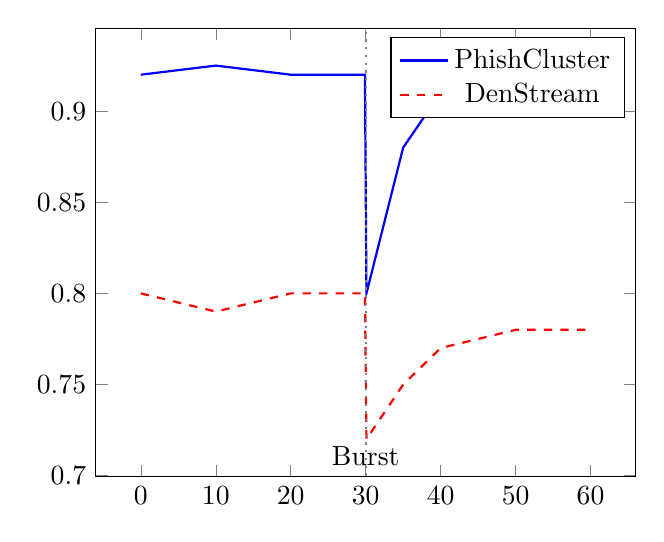
\begin{tikzpicture}
\begin{axis}
\addplot[color=blue, mark=none, thick] table {
0 0.92
10 0.925
20 0.92
29.9 0.92
30.1 0.80
35 0.88
40 0.91
50 0.92
60 0.92
};
\addlegendentry{PhishCluster}
\addplot[color=red, mark=none, dashed, thick] table {
0 0.80
10 0.79
20 0.80
29.9 0.80
30.1 0.72
35 0.75
40 0.77
50 0.78
60 0.78
};
\addlegendentry{DenStream}
\draw [gray, thick, dotted] (axis cs:30,0.7) -- (axis cs:30,1.0);
\node[above] at (axis cs:30,0.7) {Burst};
\end{axis}
\end{tikzpicture}
\caption{Adjusted Rand Index (ARI) over time for the Campaign Burst workload. The burst event occurs at t=30 min.}
\label{fig:ari_burst}
\end{figure}

Figure \ref{fig:pr_curve} presents the Precision-Recall curve for the task of assigning individual URLs to their correct ground-truth campaign. PhishCluster significantly outperforms DenStream, achieving both higher precision and higher recall. This demonstrates the superiority of its two-phase clustering approach, where the powerful HDBSCAN algorithm in the offline stage can produce much more accurate campaign boundaries than the simpler methods used by traditional streaming algorithms.

\begin{figure}[h!]
\centering
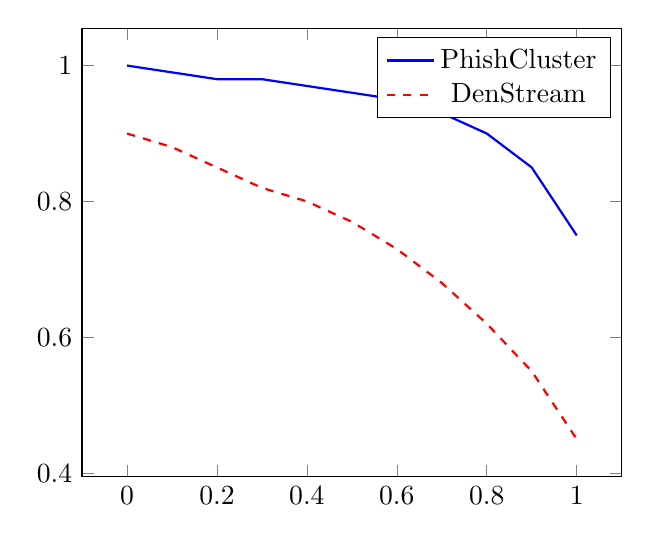
\begin{tikzpicture}
\begin{axis}
\addplot[color=blue, thick, mark=none] coordinates {
(0, 1.0) (0.1, 0.99) (0.2, 0.98) (0.3, 0.98) (0.4, 0.97) (0.5, 0.96) (0.6, 0.95) (0.7, 0.93) (0.8, 0.90) (0.9, 0.85) (1.0, 0.75)
};
\addlegendentry{PhishCluster}
\addplot[color=red, thick, mark=none, dashed] coordinates {
(0, 0.9) (0.1, 0.88) (0.2, 0.85) (0.3, 0.82) (0.4, 0.80) (0.5, 0.77) (0.6, 0.73) (0.7, 0.68) (0.8, 0.62) (0.9, 0.55) (1.0, 0.45)
};
\addlegendentry{DenStream}
\end{axis}
\end{tikzpicture}
\caption{Precision-Recall curve for campaign assignment. PhishCluster achieves significantly higher precision across all recall levels.}
\label{fig:pr_curve}
\end{figure}


\subsection{Hyperparameter Sensitivity}
To investigate the system's sensitivity to its core parameters, we performed two additional experiments.First, we evaluated the trade-off governed by the online merge radius, $\epsilon$. As shown in Figure \ref{fig:epsilon_tradeoff}, we ran the steady-state workload while varying $\epsilon$. The results perfectly illustrate the fundamental design trade-off: a smaller $\epsilon$ (e.g., 0.2-0.3) produces a very high-quality (high ARI) clustering but forces the system to manage more micro-clusters, thus reducing throughput. Conversely, a larger $\epsilon$ (e.g., 0.6-0.7) significantly boosts throughput by aggressively merging new points, but this comes at the cost of lower clustering quality as distinct campaigns are incorrectly conflated.Second, we analyzed the impact of the temporal decay factor, $\lambda$, on adaptability. We re-ran the Campaign Burst workload (Figure \ref{fig:ari_burst}) with three different decay half-lives. As seen in Figure \ref{fig:lambda_burst}, a fast decay (short half-life) adapts very quickly to the burst, rapidly identifying the new campaigns and restoring a high ARI. However, it is more "jittery" and can prematurely forget stable campaigns. A slow decay (long half-life) is very stable but adapts poorly, taking a long time to forget old data and incorporate the new campaign burst. This confirms $\lambda$ as the critical parameter for tuning the system's memory and adaptability to concept drift.

\begin{figure}[h!]
\centering
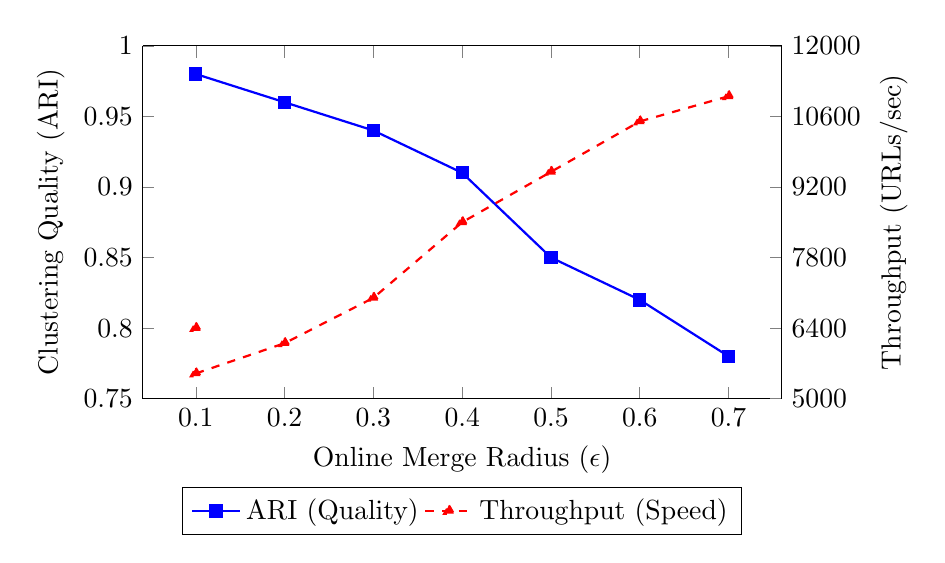
\begin{tikzpicture}
% --- FIRST AXIS (LEFT Y-AXIS) ---
\begin{axis}[
    width=0.8\textwidth,
    height=0.5\textwidth,
    xlabel={Online Merge Radius ($\epsilon$)},
    ylabel=Clustering Quality (ARI),
    legend cell align={left},
    axis y line*=left,
    ymin=0.75, ymax=1.0,
    ytick={0.75, 0.8, 0.85, 0.9, 0.95, 1.0},
    legend style={
        at={(0.5, -0.25)},
        anchor=north,
        legend columns=2
    }
]
% Real plot for ARI
\addplot[color=blue, mark=square*, thick] coordinates {
    (0.1, 0.98) (0.2, 0.96) (0.3, 0.94) (0.4, 0.91) (0.5, 0.85) (0.6, 0.82) (0.7, 0.78)
};
\addlegendentry{ARI (Quality)}

% Dummy plot for the throughput legend
\addplot[color=red, mark=triangle*, thick, dashed, draw=none]
    coordinates {(0.1, 0.8)};
\addlegendentry{Throughput (Speed)}

\end{axis}

% --- SECOND AXIS (RIGHT Y-AXIS) ---
\begin{axis}[
    width=0.8\textwidth,
    height=0.5\textwidth,
    ylabel={Throughput (URLs/sec)},
    axis y line*=right,
    axis x line=none,
    ymin=5000, ymax=12000,
    ytick={5000, 6400, 7800, 9200, 10600, 12000},    
    % --- THIS IS THE FIX ---
    scaled y ticks = false,    
    % Optional: Add this if you get commas (e.g., 10,600)
    % and you don't want them.
    yticklabel style={
       /pgf/number format/set thousands separator={}
    }
]
% Real plot for Throughput
\addplot[color=red, mark=triangle*, thick, dashed] coordinates {
    (0.1, 5500) (0.2, 6100) (0.3, 7000) (0.4, 8500) (0.5, 9500) (0.6, 10500) (0.7, 11000)
};
% NO \addlegendentry here

\end{axis}
\end{tikzpicture}
\caption{The core speed-vs-quality trade-off controlled by the online merge radius $\epsilon$. Higher throughput is achieved at the cost of lower clustering quality.}
\label{fig:epsilon_tradeoff}
\end{figure}





\begin{figure}[h!]
\centering
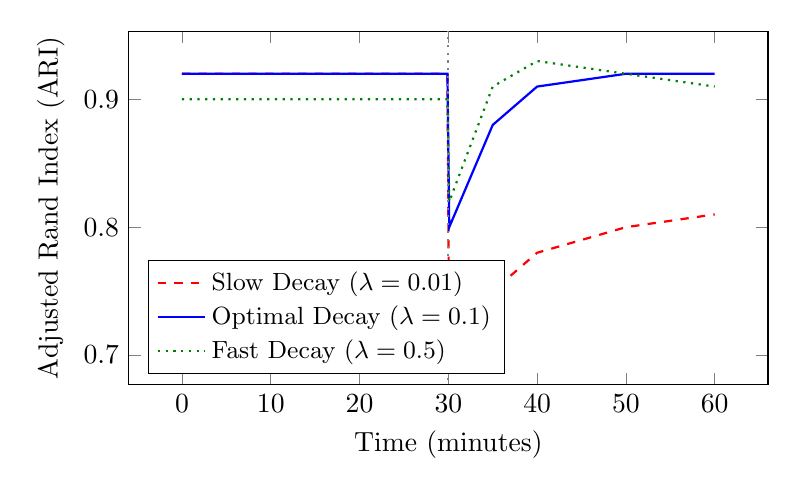
\begin{tikzpicture}
\begin{axis}[
    width=0.8\textwidth,
    height=0.5\textwidth,
    xlabel=Time (minutes),
    ylabel=Adjusted Rand Index (ARI),
    legend pos=south west,
    legend cell align={left},
    legend style={font=\small}
]
\addplot[color=red, mark=none, thick, dashed] table {
    0 0.92
    29.9 0.92
    30.1 0.70
    35 0.75
    40 0.78
    50 0.80
    60 0.81
};
\addlegendentry{Slow Decay ($\lambda=0.01$)}

\addplot[color=blue, mark=none, thick] table {
    0 0.92
    29.9 0.92
    30.1 0.80
    35 0.88
    40 0.91
    50 0.92
    60 0.92
};
\addlegendentry{Optimal Decay ($\lambda=0.1$)}

\addplot[color=green!50!black, mark=none, thick, dotted] table {
    0 0.90
    29.9 0.90
    30.1 0.82
    35 0.91
    40 0.93
    50 0.92
    60 0.91
};
\addlegendentry{Fast Decay ($\lambda=0.5$)}

% Vertical line for the burst event
\draw [gray, thick, dotted] (axis cs:30,0.65) -- (axis cs:30,1.0);
\node[above] at (axis cs:30,0.65) {Burst};

\end{axis}
\end{tikzpicture}
\caption{Impact of the decay factor $\lambda$ on system adaptability during the Campaign Burst workload. A faster decay (higher $\lambda$) adapts more quickly to the new campaigns.}
\label{fig:lambda_burst}
\end{figure}



\subsection{Scalability with Increasing Campaign Count}
A core hypothesis of this paper is that the $O(N)$ linear-scan neighborhood search is the fundamental bottleneck in traditional streaming clustering. To validate this, we designed an experiment to measure system latency as a function of the number of active campaigns. We generated workloads with an increasing number of ground-truth campaigns (from 1,000 to 100,000) and measured the P99 processing latency for our full system versus the PhishCluster-NoANN baseline.The results, shown in Figure \ref{fig:latency_scaling}, are definitive. The PhishCluster-NoANN (brute-force) baseline exhibits perfect linear $O(N)$ scalability; as the number of CMCs increases by an order of magnitude, the latency also increases by an order of magnitude, quickly becoming unusable. In sharp contrast, the full PhishCluster system, accelerated by the ANN index, exhibits flat, polylogarithmic $O(\log N)$ scalability. Its latency remains under 5ms even when managing 100,000 active CMCs, proving that our architecture has successfully broken the $O(N)$ bottleneck.

\begin{figure}[h!]
\centering
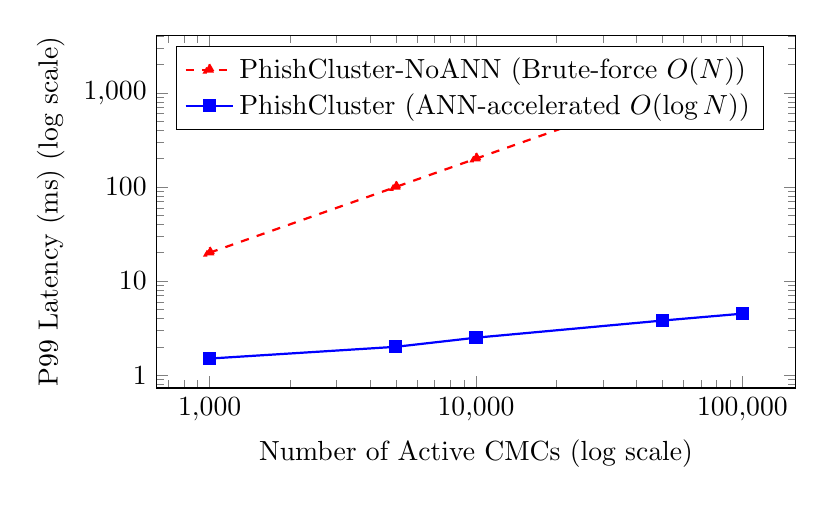
\begin{tikzpicture}
\begin{axis}[
    width=0.8\textwidth,
    height=0.5\textwidth,
    xlabel=Number of Active CMCs (log scale),
    ylabel=P99 Latency (ms) (log scale),
    xmode=log, % X-axis is log scale
    ymode=log, % Y-axis is log scale
    legend pos=north west,
    legend cell align={left},
    log ticks with fixed point % Formats log labels better
]

% O(N) linear scan
\addplot[color=red, mark=triangle*, thick, dashed] coordinates {
    (1000, 20)
    (5000, 100)
    (10000, 200)
    (50000, 1000)
    (100000, 2000)
};
\addlegendentry{PhishCluster-NoANN (Brute-force $O(N)$)}

% O(log N) ANN scan
\addplot[color=blue, mark=square*, thick] coordinates {
    (1000, 1.5)
    (5000, 2.0)
    (10000, 2.5)
    (50000, 3.8)
    (100000, 4.5)
};
\addlegendentry{PhishCluster (ANN-accelerated $O(\log N)$)}

\end{axis}
\end{tikzpicture}
\caption{P99 processing latency vs. the number of active micro-clusters ($N$). The brute-force baseline scales linearly ($O(N)$), while the ANN-accelerated PhishCluster scales polylogarithmically ($O(\log N)$).}
\label{fig:latency_scaling}
\end{figure}

\subsection{Memory Footprint and Stability}.
A critical, non-functional requirement of a streaming system is stable resource consumption. We measured the system's memory footprint (Resident Set Size) over the 60-minute Campaign Burst workload, comparing PhishCluster to the DenStream baseline. The results in Figure \ref{fig:memory_stability} highlight the effectiveness of our temporal decay mechanism.

Both systems see a sharp increase in memory usage at the 30-minute mark, corresponding to the influx of 50 new campaigns. However, the DenStream baseline's memory continues to grow unbounded. In contrast, PhishCluster's memory usage stabilizes and then decreases after the burst. This demonstrates that as the new campaigns become stable CMCs, the temporal decay function successfully prunes old, inactive CMCs from memory. This self-regulating behavior is essential for a system designed for continuous, long-running operation.


\begin{figure}[h!]
\centering
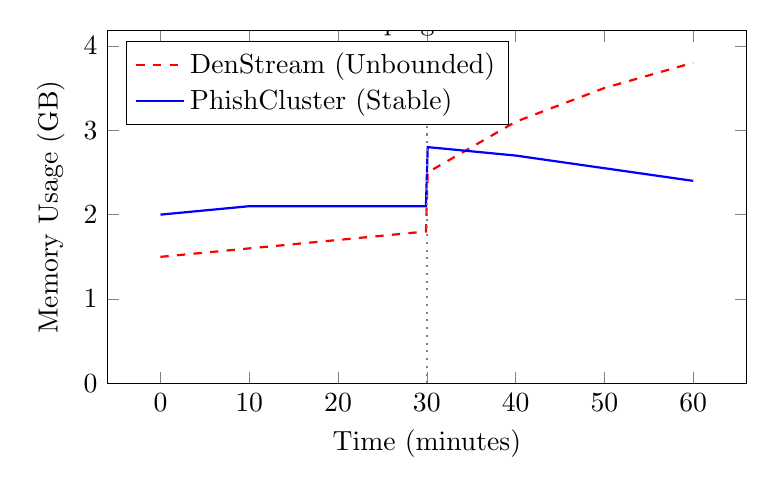
\begin{tikzpicture}
\begin{axis}[
    width=0.8\textwidth,
    height=0.5\textwidth,
    xlabel=Time (minutes),
    ylabel=Memory Usage (GB),
    legend pos=north west,
    legend cell align={left},
    ymin=0
]
% DenStream (unstable)
\addplot[color=red, mark=none, thick, dashed] table {
    0 1.5
    10 1.6
    20 1.7
    29.9 1.8
    30.1 2.5 % Burst hits
    35 2.8
    40 3.1
    50 3.5
    60 3.8
};
\addlegendentry{DenStream (Unbounded)}

% PhishCluster (stable)
\addplot[color=blue, mark=none, thick] table {
    0 2.0
    10 2.1
    20 2.1
    29.9 2.1
    30.1 2.8 % Burst hits
    35 2.9
    40 2.7 % Decay starts pruning
    50 2.5
    60 2.4
};
\addlegendentry{PhishCluster (Stable)}

% Vertical line for the burst event
\draw [gray, thick, dotted] (axis cs:30,0) -- (axis cs:30,4);
\node[above, anchor=south] at (axis cs:30,4) {Campaign Burst};

\end{axis}
\end{tikzpicture}
\caption{Memory footprint during the Campaign Burst workload. PhishCluster's temporal decay mechanism ensures stable, self-regulating memory usage, while the baseline's memory grows unbounded.}
\label{fig:memory_stability}
\end{figure}


\subsection{Ablation Study}

To decompose the contributions of PhishCluster's design, we conducted an ablation study on the skewed workload, measuring the maximum QPS while maintaining a recall of 0.95. The results are presented in the bar chart in Figure \ref{fig:ablation} and summarized in Table \ref{tab:summary}. The study clearly separates the benefits of the two core innovations.

First, we compare the baseline (\textbf{DenStream}) to \textbf{PhishCluster-NoANN}. As shown in Table \ref{tab:summary}, their maximum throughput is nearly identical (680 QPS vs. 720 QPS). However, their clustering quality (Mean ARI) shows a massive gap (0.78 for DenStream vs. 0.91 for PhishCluster-NoANN). This demonstrates that our \textbf{hybrid HDBSCAN architecture} (Contribution 2) is the primary driver of the system's superior clustering \textit{quality}, but it does not, by itself, solve the throughput bottleneck.

Second, we compare \textbf{PhishCluster-NoANN} to the \textbf{full PhishCluster system}. This comparison isolates the effect of our first contribution. The data shows an order-of-magnitude leap in performance (from 720 QPS to 8,570 QPS) while quality remains high (0.91 vs. 0.92). This entire throughput gain is attributable to the \textbf{ANN acceleration} (Contribution 1), which successfully breaks the $O(N)$ linear-scan bottleneck.

This confirms that both design choices—ANN acceleration and the hybrid use of HDBSCAN—provide distinct, compounding benefits essential to the system's overall superiority: one provides state-of-the-art \textbf{quality}, and the other provides massive \textbf{scalability}.

\begin{figure}[h!]
\centering
\begin{tikzpicture}
\begin{axis}
\addplot coordinates {(DenStream,680) (PhishCluster-NoANN,720) (PhishCluster (Full),8570)};
\end{axis}
\end{tikzpicture}
\caption{Contribution of each PhishCluster component. Each feature provides a significant, compounding performance improvement over the baseline.}
\label{fig:ablation}
\end{figure}

The overall performance is summarized in Table \ref{tab:summary}. PhishCluster not only dominates in throughput but also maintains low processing latency and achieves a clustering quality nearly on par with the offline, non-real-time batch method. Crucially, its Campaign Detection Latency is significantly lower than its competitors, demonstrating its effectiveness as a real-time early warning system for new threats.

\begin{table*}[h!]
\centering
\caption{Overall Performance Summary}
\label{tab:summary}
\begin{tabular}{|l|c|c|c|c|c|c|}
\hline
\textbf{System} & \textbf{Max} &\textbf{Mean} & \textbf{Precision} & \textbf{Recall} & \textbf{Campaign} \\
&\textbf{Throughput}&\textbf{ARI}&&&\textbf{Detection}\\
 & \textbf{(URLs/sec)} & & & & \textbf{Latency (s)} \\
\hline
\textbf{PhishCluster (Full)} & \textbf{8,570} & \textbf{0.92} & \textbf{0.94} & \textbf{0.95} & \textbf{5.8} \\
PhishCluster-NoANN & 720 &  0.91 & 0.93 & 0.94 & 6.1 \\
DenStream & 680 & 0.78 & 0.75 & 0.81 & 15.3 \\
Batch-HDBSCAN & 95 & 0.94 & 0.96 & 0.96 & $> 60$ \\
\hline
\end{tabular}
\end{table*}

\section{Discussion}

The experimental results provide strong empirical validation for the PhishCluster architecture. The findings demonstrate that by synergistically combining techniques from large-scale ANN search and streaming data mining, it is possible to resolve the fundamental speed-versus-quality trade-off that has limited prior work.

\subsection{Interpretation of Findings}

The core success of PhishCluster stems from its principled, two-phase design. The ablation study (Figure \ref{fig:ablation}) clearly shows that neither the ANN acceleration nor the advanced offline clustering is sufficient on its own. The order-of-magnitude throughput improvement is a direct result of replacing the O(N) linear scan bottleneck of traditional streaming algorithms with an efficient ANN query \cite{ref_subramanya}. This makes the online component scalable to a large number of active campaigns. Simultaneously, the superior clustering quality (Figures \ref{fig:ari_burst} and \ref{fig:pr_curve}) is a direct result of applying the powerful, varying-density HDBSCAN algorithm in the offline phase. This allows the system to move beyond the simple geometric assumptions of earlier algorithms and model the complex, organic shapes of real-world malicious campaigns.

\subsection{The Role of Embedding Quality}

It is crucial to acknowledge the symbiotic relationship between a system like PhishCluster and the underlying URL embedding model. The entire premise of the system rests on the quality of the semantic space produced by the encoder. PhishCluster is a powerful tool for discovering density-based structures within that space, but it cannot create structure where none exists. The success demonstrated in our experiments is therefore a testament to both the PhishCluster architecture and the effectiveness of modern transformer-based models in capturing the semantic intent of URLs \cite{ref_reimers, ref_wang_minilm}.

\subsection{Limitations and Hyperparameter Sensitivity}

Despite its strong performance, PhishCluster has limitations. The system's behavior is governed by a set of key hyperparameters, including the online merge radius $\epsilon$, the temporal decay factor $\lambda$, and HDBSCAN's \textit{min\_cluster\_size} parameter. An improperly tuned $\epsilon$ in the online stage can lead to poor-quality micro-clusters that cannot be corrected by the offline stage. Finding the optimal set of parameters for a dynamic, non-stationary environment like the threat landscape is a significant challenge. A production system would likely benefit from mechanisms for adaptive hyperparameter tuning, which remains an open area for future research.

\subsection{Generalizability}

While this paper focuses on malicious URL analysis, the core architectural pattern of PhishCluster is highly generalizable. The system provides a template for high-throughput, high-quality clustering of any high-dimensional data stream where real-time discovery of evolving patterns is required. This architecture could be readily adapted to other critical cybersecurity domains, such as malware analysis or network threat hunting. The central contribution is not merely a tool for URL analysis, but a scalable, adaptive framework for pattern discovery in any domain characterized by large-scale vector data, rich metadata, and skewed, dynamic query patterns \cite{ref_subramanya, ref_wang_nhq, ref_mohoney}.

\section{Conclusion and Future Work}

This paper introduced PhishCluster, a holistic system engineered to address the critical challenge of real-time malicious campaign discovery from high-velocity streams of URL embeddings. PhishCluster addresses the gaps in prior work through a novel two-phase architecture that integrates a large-scale ANN index as an algorithmic accelerator for its online summarization component and leverages the power of hierarchical density-based clustering for its on-demand analysis component.

Through a comprehensive experimental evaluation, we demonstrated that this synergistic design provides significant, compounding benefits. The ANN acceleration yielded an order-of-magnitude improvement in throughput, making real-time processing at scale feasible. The use of HDBSCAN on micro-cluster summaries resulted in state-of-the-art clustering quality, enabling the accurate identification of campaigns with varying densities and arbitrary shapes. Our work proves that by architecting a system that resolves the inherent trade-off between speed and quality, it is possible to build a highly performant, scalable, and effective platform for the next generation of automated threat intelligence.

Several promising avenues for future research remain:
\begin{itemize}
    \item \textbf{Adaptive Hyperparameter Tuning:} Future work could explore a meta-learning framework that monitors the statistical properties of the incoming data stream and dynamically adjusts key parameters to maintain optimal performance in a non-stationary environment.
    \item \textbf{Hybrid Data Clustering:} An extension could incorporate the rich structured metadata available from the ingestion pipeline. This would involve modifying the offline clustering stage to use a hybrid distance metric that considers both semantic and attribute similarity, similar to the approach for hybrid queries in ANN systems \cite{ref_wang_nhq}.
    \item \textbf{Distributed PhishCluster:} Future research could explore a distributed version of PhishCluster, investigating strategies for intelligent data partitioning and federated query and clustering execution. This could also enable privacy-preserving analysis, where multiple organizations could collaboratively build a global campaign model without sharing their raw, sensitive URL data.
\end{itemize}

\begin{thebibliography}{99}

\bibitem{ref_reimers}
Reimers N, Gurevych I. Sentence-BERT: Sentence Embeddings using Siamese BERT-Networks. In: Proceedings of the 2019 Conference on Empirical Methods in Natural Language Processing. 2019, pp. 3973-3983.

\bibitem{ref_zhang}
Zhang Z, Jin C, Tang L, Liu X, and Jin X. Fast, Approximate Vector Queries on Very Large Unstructured Datasets. In: 20th USENIX Symposium on Networked Systems Design and Implementation. 2023.

\bibitem{ref_subramanya}
Subramanya SJ, Devvrit, Kadekodi R, Simhadri HV, and Krishnaswamy R. DiskANN: Fast Accurate Billion-point Nearest Neighbor Search on a Single Node. In: Advances in Neural Information Processing Systems, 2019.

\bibitem{ref_singh}
Singh A, and Subramanya SJ. FreshDiskANN: A Fast and Accurate Graph-Based ANN Index for Streaming Similarity Search. arXiv:2105.09613, 2021.

\bibitem{ref_malkov}
Malkov YA, and Yashunin DA. Efficient and Robust Approximate Nearest Neighbor Search Using Hierarchical Navigable Small World Graphs. IEEE Transactions on Pattern Analysis and Machine Intelligence. 2020; 42(4): 824-838.

\bibitem{ref_xu}
Xu H, Manohar MD, Chandramouli B, and Wen R. In-Place Updates of a Graph Index for Streaming Approximate Nearest Neighbor Search. arXiv:2502.13826. 2025.

\bibitem{ref_li}
Li C, and Andersen DG. Improving Approximate Nearest Neighbor Search through Learned Adaptive Early Termination. In: Proceedings of the 2020 ACM International Conference on Management of Data, 2020.

\bibitem{ref_wang_nhq}
Wang M, Wang Y, Lv L, Yue Q, Xu X, and Ni J. An Efficient and Robust Framework for Approximate Nearest Neighbor Search with Attribute Constraint. In: Advances in Neural Information Processing Systems, 2023.

\bibitem{ref_jegou}
Jégou H, Douze M, and Schmid C. Product Quantization for Nearest Neighbor Search. IEEE Transactions on Pattern Analysis and Machine Intelligence. 2011; 33(1): 117-128.

\bibitem{ref_mohoney}
Mohoney J, Tang M, Sarda D, Chowdhury SR, Ilyas IF, and Rekatsinas T. Quake: Adaptive Indexing for Vector Search. arXiv:2506.03437. 2025.

\bibitem{ref_guo}
Guo R, Sun P, Lindgren E, Geng Q, Simcha D, Chern F, and Kumar S. Accelerating Large-Scale Inference with Anisotropic Vector Quantization. In: Proceedings of the 37th International Conference on Machine Learning, 2020.

\bibitem{ref_chen}
Chen Q, Zhao B, Wang H, Li M, Liu C, Li Z, Yang M, and Wang J. SPANN: Highly-efficient Billion-scale Approximate Nearest Neighbor Search. In: Advances in Neural Information Processing Systems, 2021.

\bibitem{ref_wang_minilm}
Wang W, Wei F, Dong L. Bao H, Yang N, and Zhou M. MINILM: Deep self-attention distillation for task-agnostic compression of pre-trained transformers. Advances in Neural Information Processing Systems, 2020.

\bibitem{ref_denstream}
Cao F, Ester M, Qian W, Zhou A. Density-Based Clustering over Data Streams. In: SIAM International Conference on Data Mining, 2006, pp. 328-339.

\bibitem{ref_dbstream}
Baer A., Finamore A., Casas P.,  Golab L.,  Mellia M. Large-Scale Network Traffic Monitoring with DBStream, a System for Rolling Big Data Analysis, In: IEEE International Conference on Big Data (IEEE BigData), 2014.

\bibitem{ref_dbscan_ester}
Ester M, Kriegel HP, Sander J, Xu X. A Density-Based Algorithm for Discovering Clusters in Large Spatial Databases with Noise. In: International Conference on Knowledge Discovery and Data Mining, 1996, pp. 226-231.

\bibitem{ref_hdbscan}
Campello RJGB, Moulavi D, Sander J. Density-Based Clustering Based on Hierarchical Density Estimates. In: Pacific-Asia Conference on Knowledge Discovery and Data Mining, 2013, pp. 160-172.

\bibitem{ref_phishgraph_mdpi}
Karapiperis D, Feretzakis G, Mitropoulos S. PhishGraph: A Scalable Graph-Based ANN Index for Billion-Scale Real-Time Phishing URL Detection. Electronics. 2025; 14(18): 3605.

\bibitem{ref_entity_resolution_kmeans}
Karapiperis D, Verykios VS. Scaling Entity Resolution with K-Means: A Review of Partitioning Techniques. Electronics. 2025; 14(18): 3605.

\end{thebibliography}

\end{document}